\documentclass[final]{IEEEtran}
%\usepackage[dvips]{epsfig}
\usepackage[english]{babel}
\usepackage{graphicx}% Include figure files
\usepackage{subfigure} %��Ҫʹ�õĺ��
\usepackage{amsfonts}
%\usepackage[dvips]{graphicx}
\usepackage{multirow}
\usepackage{array}
\usepackage{amsmath}
\usepackage{url}
\usepackage{slashbox}
\usepackage{diagbox}
\usepackage{amssymb}
\usepackage{fancyhdr}
\usepackage[T1]{fontenc}
\usepackage{mathptmx}
\def\BibTeX{{\rm B\kern-.05em{\sc i\kern-.025em b}\kern-.08em
    T\kern-.1667em\lower.7ex\hbox{E}\kern-.125emX}}

\newtheorem{theorem}{Theorem}
\newtheorem{lemma}{Lemma}
\newtheorem{pf}{Proof}
\newtheorem{definition}{Definition}
\setcounter{page}{1}


\begin{document}
\begin{figure*}[htbp]
\begin{minipage}[t]{0.33\linewidth}
\centering
 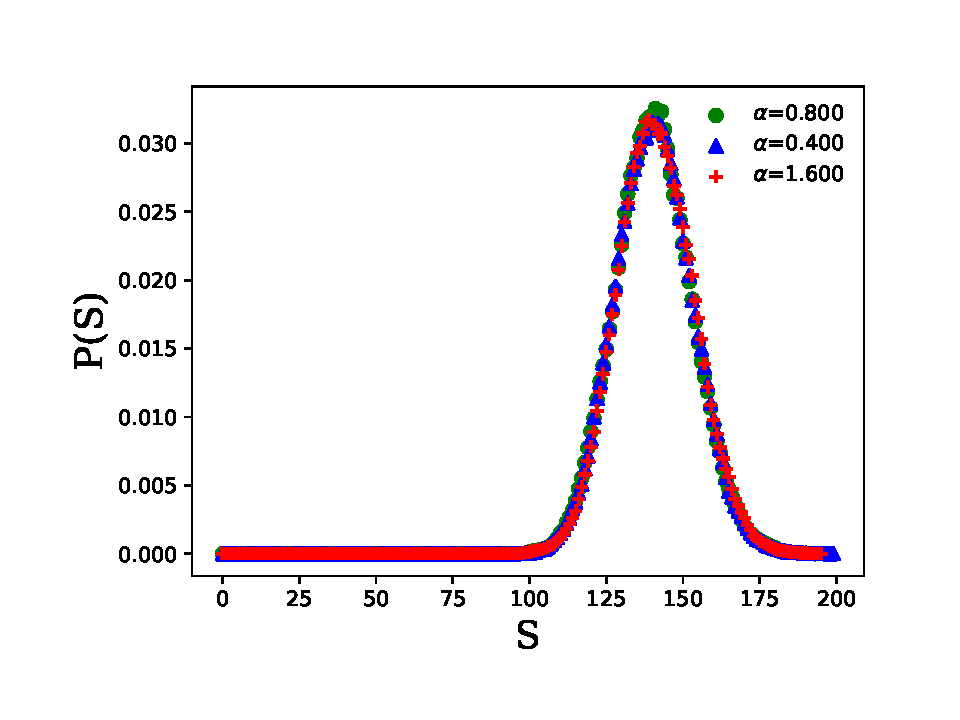
\includegraphics[height=4.4cm, width=6.6cm]{dd(1)}
\parbox{4.4cm}\centering{\footnotesize \hspace{0.1cm}(a) The distribution of $S$ individual number with different values of $\alpha$}

\end{minipage}
\begin{minipage}[t]{0.33\linewidth}
\centering
 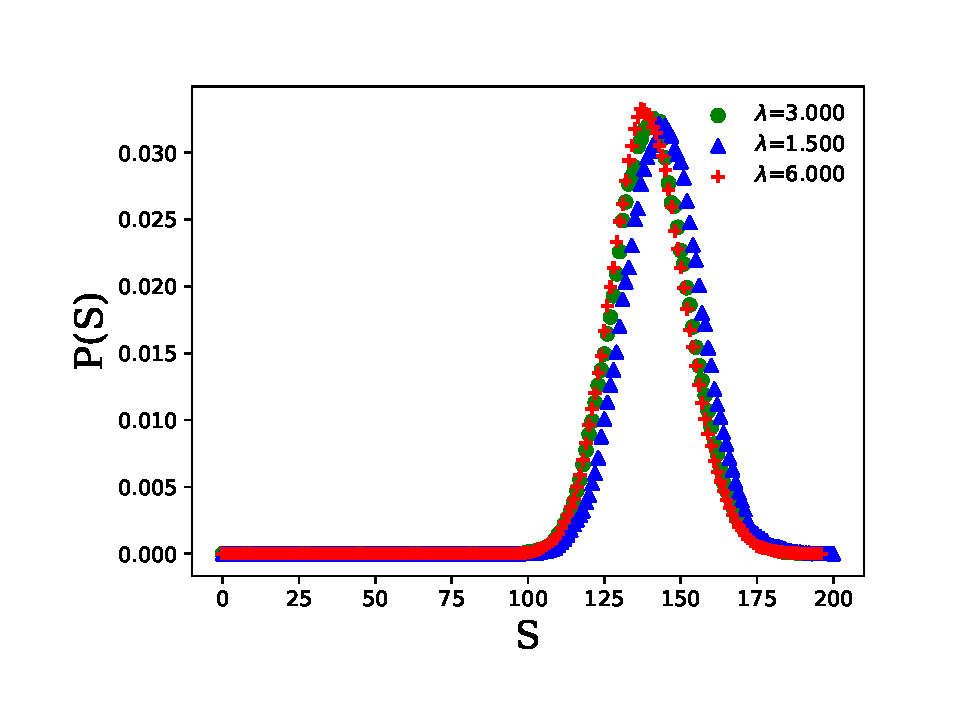
\includegraphics[height=4.4cm, width=6.6cm]{dd(7)}
\parbox{4.4cm}\centering{\footnotesize \hspace{0.1cm}(b) The distribution of $S$ individual number with different values of $\lambda$}

\end{minipage}
\begin{minipage}[t]{0.33\linewidth}
\centering
 %\epsfig{file=40,50, height=4.8cm, width=8.8cm}
 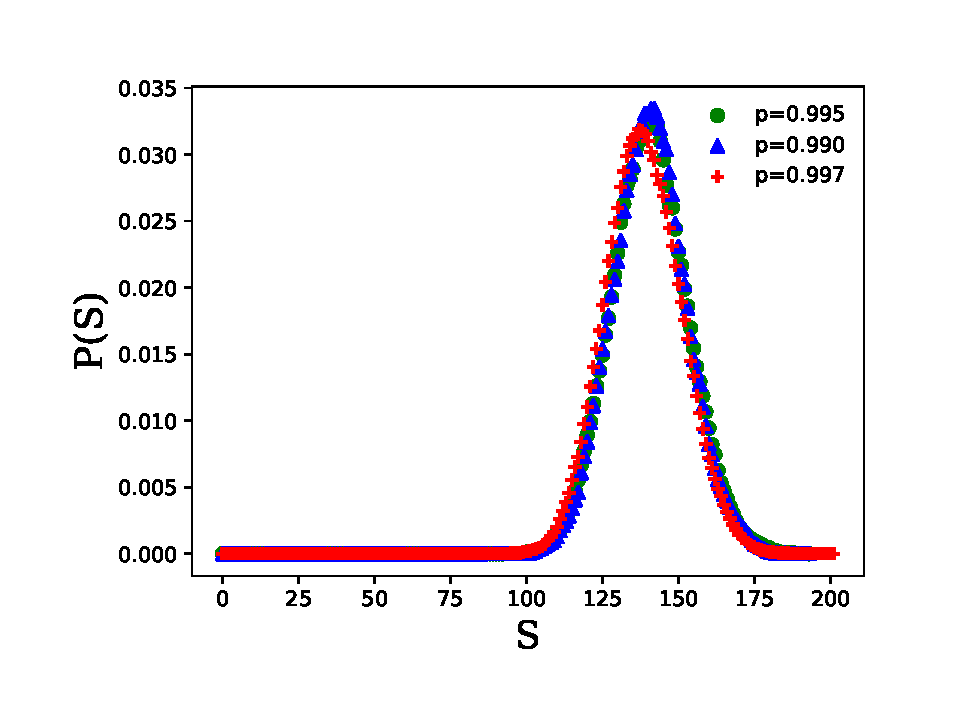
\includegraphics[height=4.4cm, width=6.6cm]{dd(10)}
\parbox{4.4cm}\centering{\footnotesize \hspace{0.1cm}(c) The distribution of $S$ individual number with different values of $p$}

\end{minipage}
\begin{minipage}[t]{0.5\linewidth}
\centering
 %\epsfig{file=40,50, height=4.8cm, width=8.8cm}
 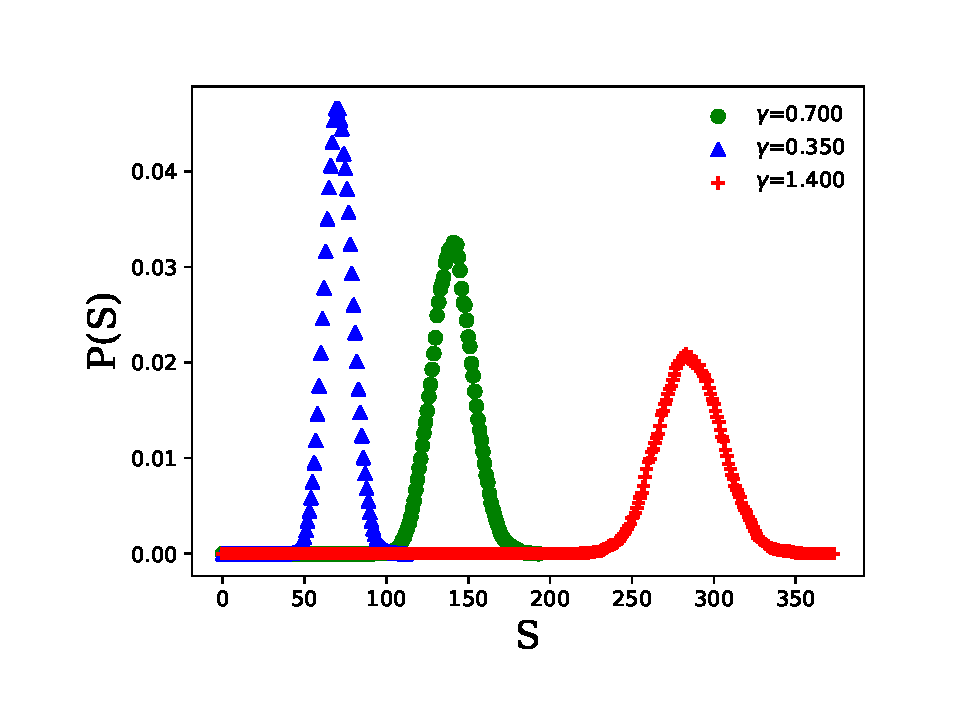
\includegraphics[height=4.4cm, width=6.6cm]{dd(4)}
\parbox{8.5cm}{\footnotesize \hspace{0.1cm}(d) The distribution of $S$ individual number with different values of $\gamma$}

\end{minipage}
\begin{minipage}[t]{0.5\linewidth}
\centering
 %\epsfig{file=40,50, height=4.8cm, width=8.8cm}
 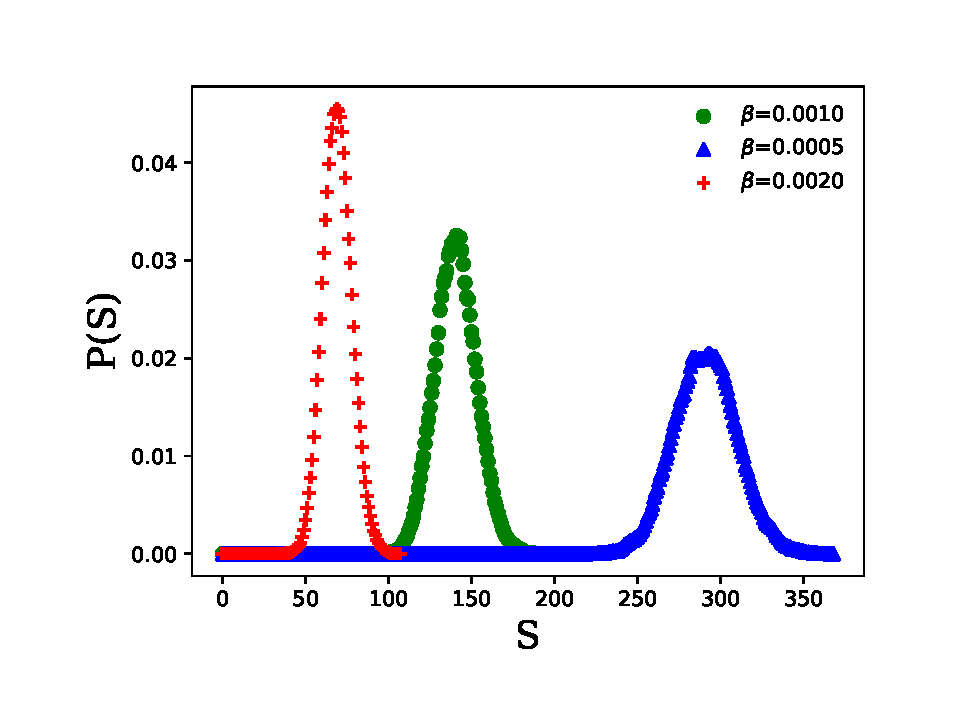
\includegraphics[height=4.4cm, width=6.6cm]{dd(16)}
\parbox{8.5cm}{\footnotesize \hspace{0.1cm}(e) The distribution of $S$ individual number with different values of $\beta$}

\end{minipage}
\end{figure*}
\end{document}